\subsection{A small bump}
On June 2nd 2015, the day before CMS recorded its first ever 13 TeV event, a pre-print appeared on the arXiv "Search for high-mass diboson resonances with boson-tagged jets in proton-proton collisions at $\sqrt{s} = 8$ \TeV with the ATLAS detector"~\cite{Aad2015}.
It was an analysis of the full ATLAS Run 1 dataset, corresponding to 20.3 \fbinv, searching for heavy resonances decaying to vector bosons in the all-hadronic state. The analysis documented a 3.4 $\sigma$ excess for a heavy resonance decaying to \PW\PZ around 2 \TeV.
The corresponding CMS analysis, published the previous year, had a 1.3 $\sigma$ excess at roughly the same resonance mass, but mostly compatible with a \PW\PW final state hypothesis~\cite{Khachatryan:1700394}. Figure~\ref{fig:searchI:8tev} shows the corresponding dijet invariant mass spectrum as seen by ATLAS (left) and the upper limit on the production times the cross section for a $G_{Bulk}$ decaying to \PW\PW (right)  as documented by CMS.

\begin{figure}[ht] 
    \centering
    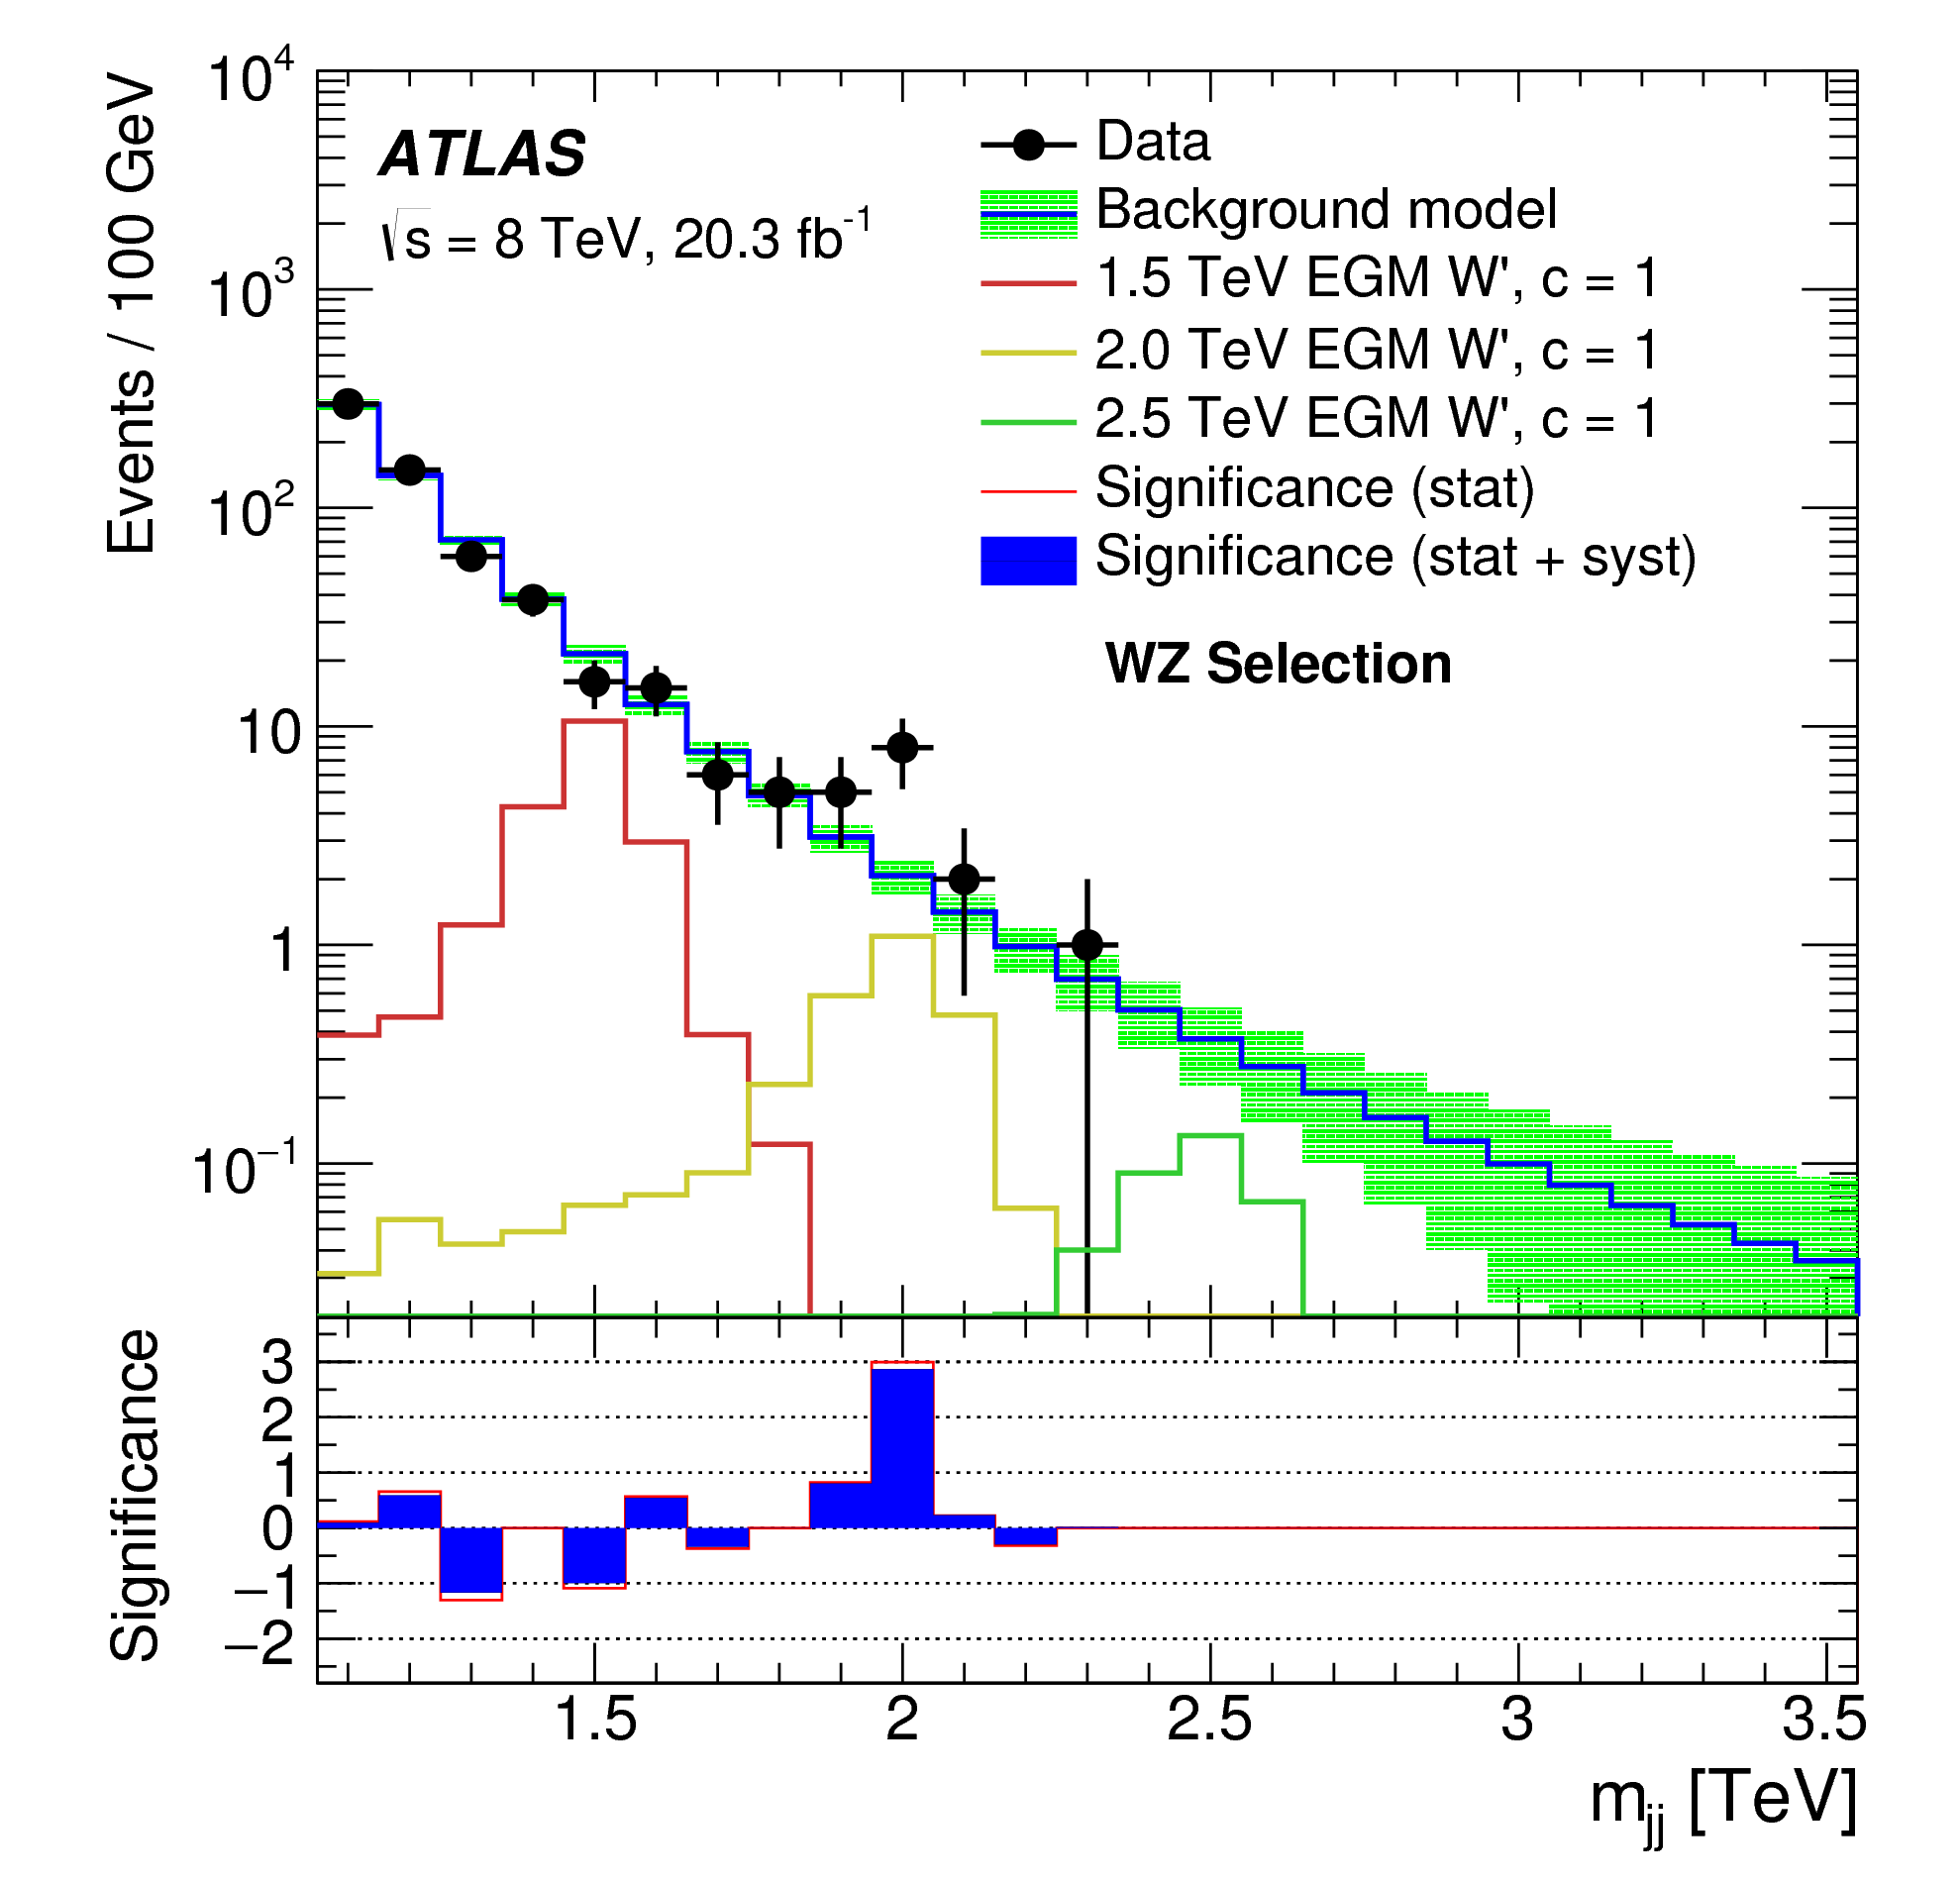
\includegraphics[width=0.4\textwidth]{figures/analysis/search1/misc/atlas_8tev.png}
    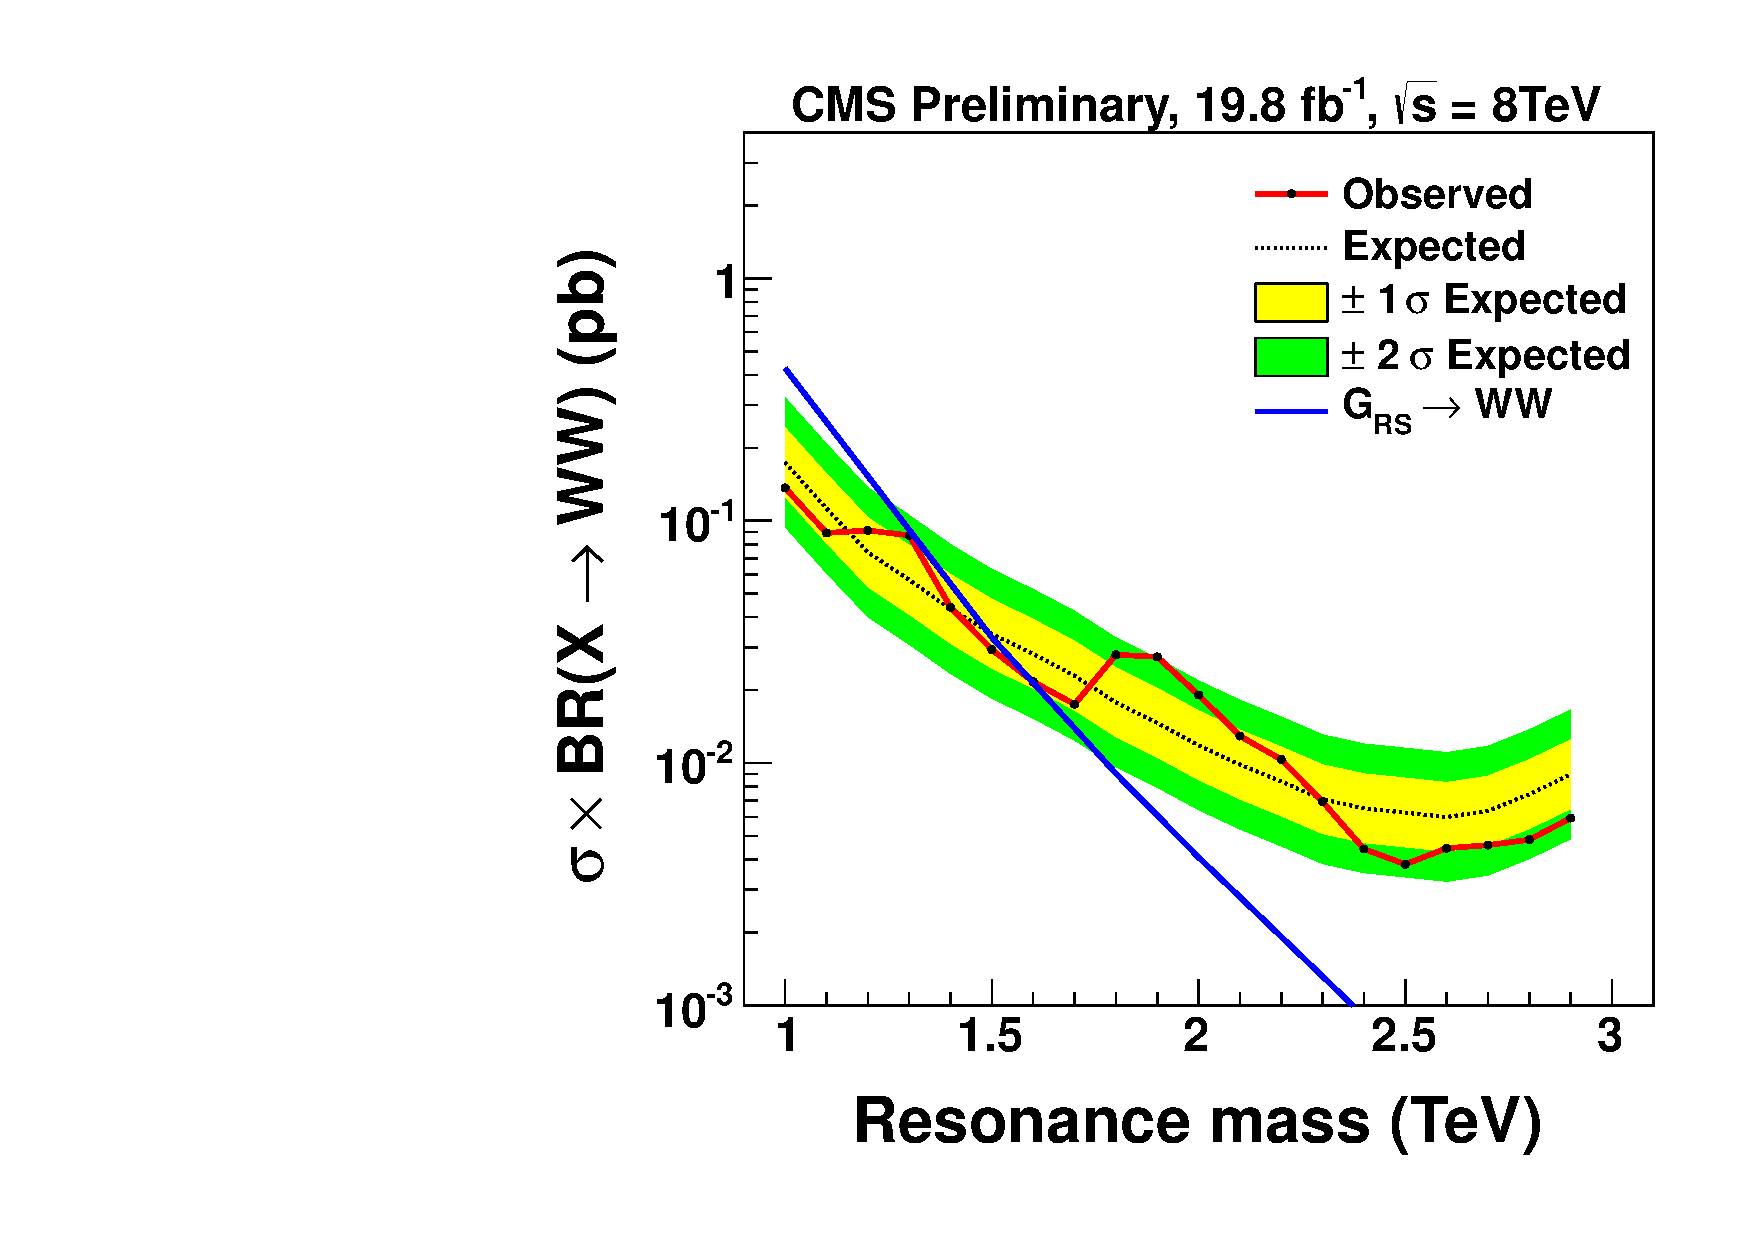
\includegraphics[width=0.4\textwidth]{figures/analysis/search1/misc/EXO-12-024_gWW.pdf}
    \caption{The mass (top) and \PT (bottom) resolution comparing PF only (blue), PF+CHS (red) and PUPPI (pink) jets. The absolute resolution (left) as well as the resolution as a function of the number of reconstructed primary vertices in the event (right)is shown~\cite{Bertolini2014}.}
    \label{fig:searchI:8tev}
\end{figure}

The two measurements were found to be compatible, favoring a heavy resonance with a production cross section of around 5 \fbinv and a mass between 1.9 and 2.0 TeV decaying to either \PW\PW, \PW\PZ or \PZ\PZ~\cite{Dias:2015mhm}. Figure~\ref{fig:searchI:8tevcombo} show the obtained p-value of the ATLAS (red) and CMS (blue) search as well as their combination (black).  

\begin{figure}[ht] 
    \centering
    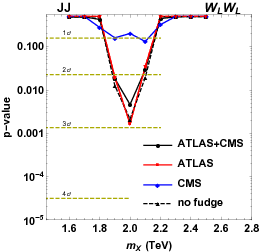
\includegraphics[width=0.25\textwidth]{figures/analysis/search1/misc/CMS_ATLAS_BulkWW_JJ_dijetfit_p.png}
    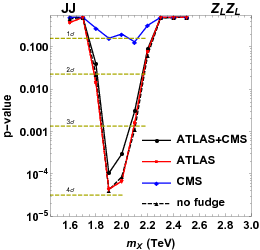
\includegraphics[width=0.25\textwidth]{figures/analysis/search1/misc/CMS_ATLAS_BulkZZ_JJ_dijetfit_p.png}
    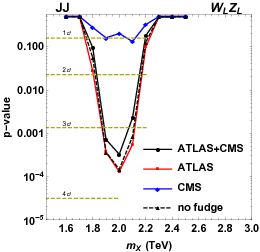
\includegraphics[width=0.25\textwidth]{figures/analysis/search1/misc/CMS_ATLAS_WZ_JJ_dijetfit_p.png}
    \caption{p-values as a function of resonance mass obtained with an emulation of the ATLAS (red) and CMS (blue) searches as well as the combination of the two (black). Here for a \PW\PW (left), \PW\PZ (middle) and \PZ\PZ (right) hypothesis~\cite{Dias:2015mhm}.}
    \label{fig:searchI:8tevcombo}
\end{figure}

The combination of the two excesses and the timing of the ATLAS paper, naturally lead to quite a commotion. And in the coming weeks, the arXiv was flooded with theory papers seeking an explanation for the measurements.
The pressure on seeing early results with 13 TeV data in the VV all-hadronic final state was high, and it was agreed with CMS Physics Coordination that a preliminary analysis would be ready in December that same year, only 6 months after the first 13 TeV collision.

\subsection{Analysis strategy}

When a resonance X with a mass above 1 TeV decays into a vector boson pair, the bosons have a very high energy ($\tilde\PT=\mX/2=500 \GeV$, assuming X is produced at rest). The boson is co-called "boosted". The decay products of a hadronically decaying boosted vector boson, will therefore not appear as back-to-back in the lab frame but rather be very collimated, as described in Section~\ref{sec:objreco:substructure}. This results in a final state with two large high-\PT jets, where an AK R=0.8 jet is expected to fully contain the two quarks coming from the vector boson decay. This is illustrated in Figure~\ref{fig:searchI:merged}.

\begin{figure}[ht] 
    \centering
    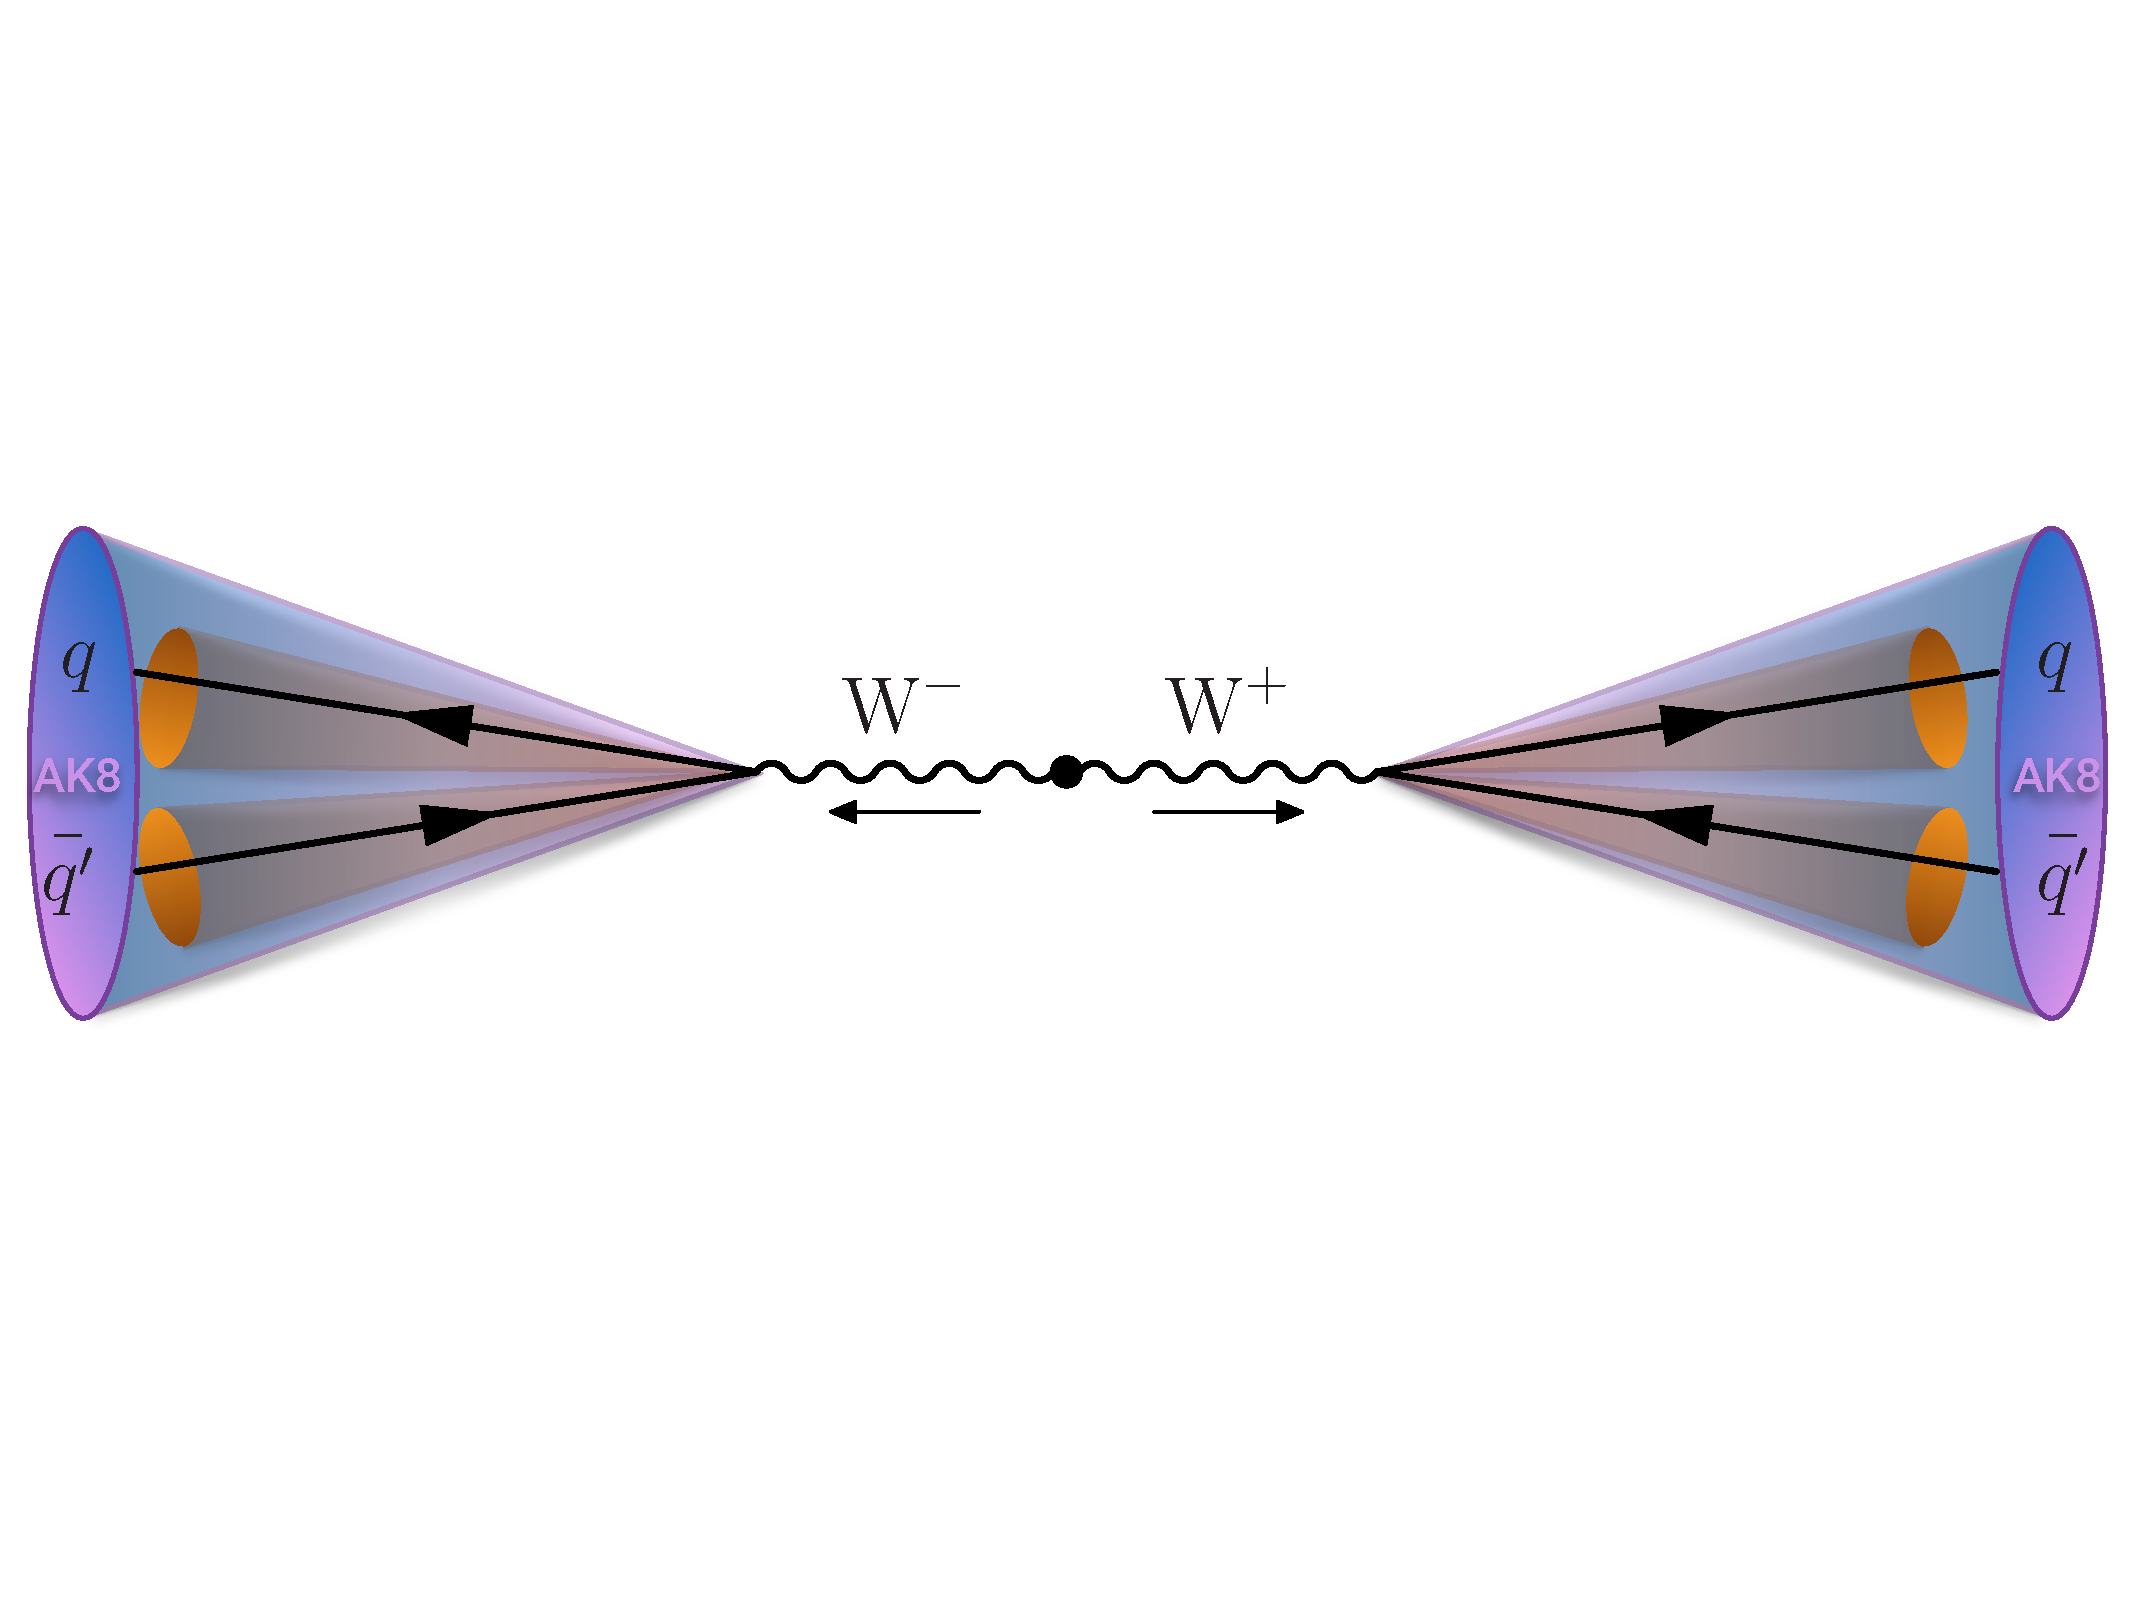
\includegraphics[width=0.70\textwidth]{figures/event_reconstruction/WWqqqq_merged_small.pdf}
    \caption{If a heavy ($>1 \TeV$) resonance decays into vector bosons, the transverse momentum of each boson will be large and its decay products are merged into one single large cone AK8 jet.}
    \label{fig:searchI:merged}
\end{figure}

The two jets are both expected to have a mass around the \PW of \PZ mass, and some intrinsic substructure stemming from their two-prong origin. The invariant mass of the dijet system, \mjj, should be roughly equal to the resonance mass \mX. This dijet system is the final state under scrutiny and the dijet invariant mass is the parameter of interest. Both \WW and \ZZ, as well as \WZ final states are of interest. \par

The main background for such an analysis, is QCD multijet events. As mentioned in Section~\ref{sec:objreco:substructure}, quark/gluon jets can obtain a high mass due to diffuse radiation and QCD processes have such a large cross section that the number of QCD jets with a mass compatible with the W mass can be large. In order to discriminate between the two, we take advantage of three properties: 1. The groomed mass of signal and background jets should be very different, 2. signal jets should appear two-prong like, quark/gluon jets not, and 3. the dijet invariant mass for a signal process should peak around the resonance mass while the QCD spectrum is predicted to be smoothly falling (we will get back to why this assumption is justified in Section~\ref{sec:searchI:bkg}). The strategy therefore consists of performing a smoothness test on \mjj of the observed data, a so-called "bump-hunt", by assuming that the signal will appear as a bump on top of a smooth distribution. This is illustrated in Figure~\ref{fig:searchI:bumphunt}.

\begin{figure}[ht] 
    \centering
    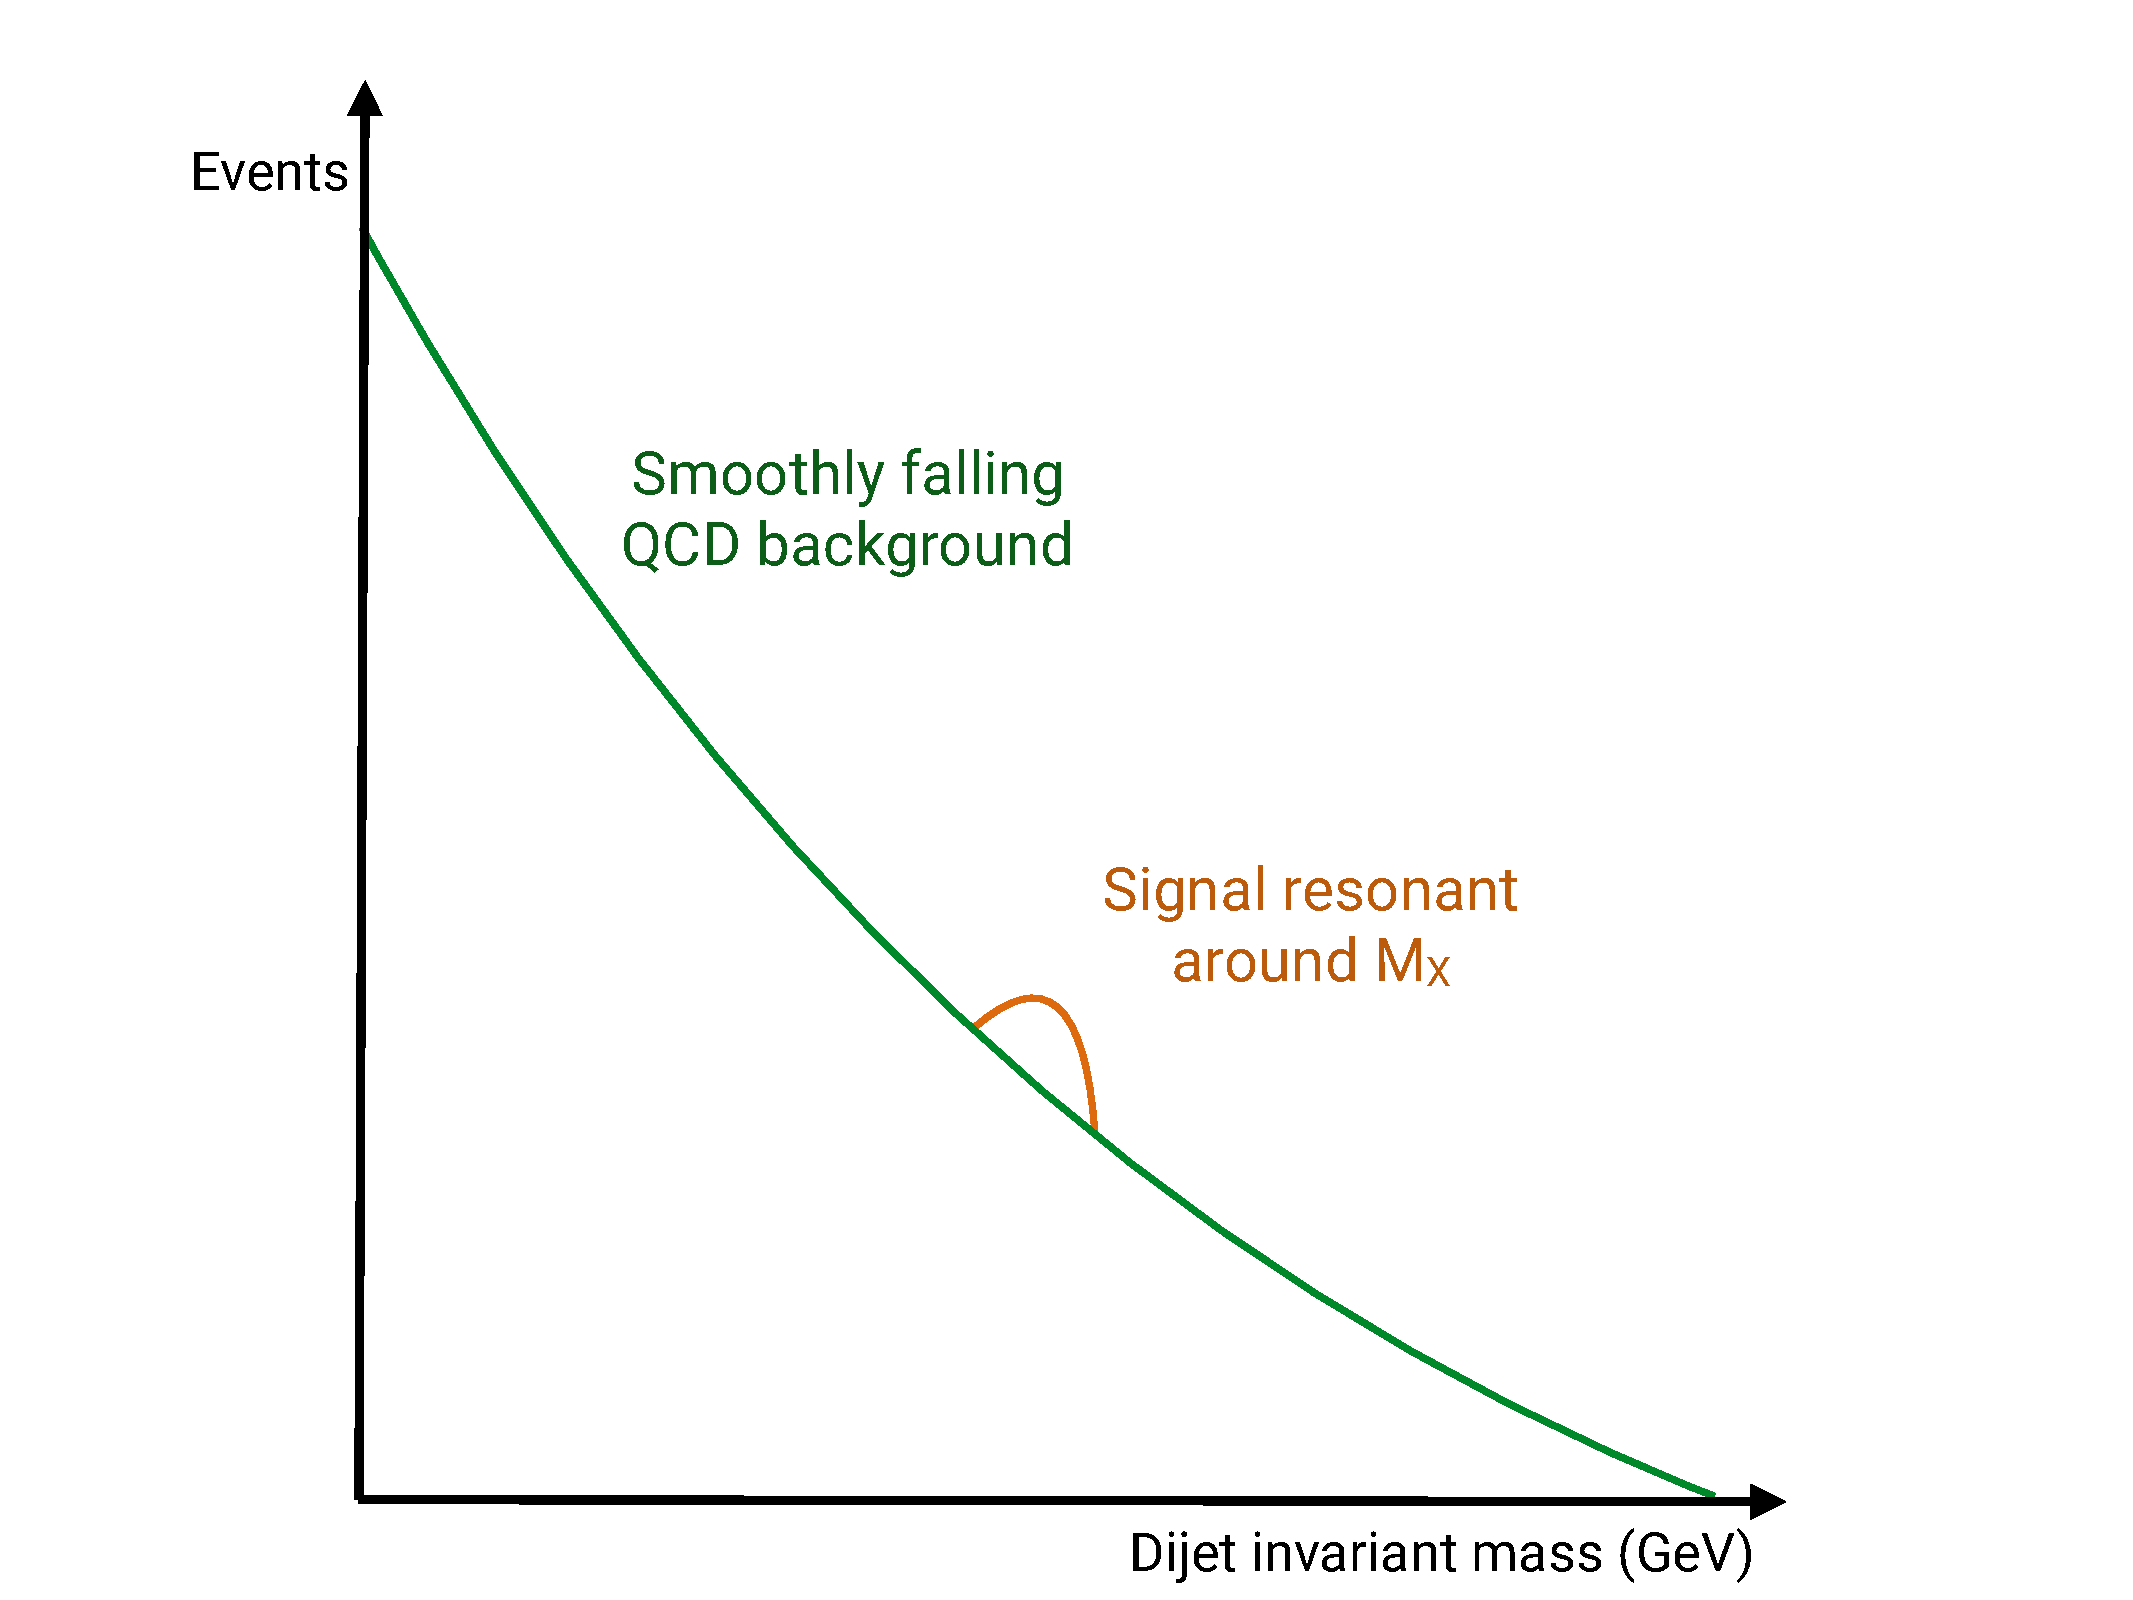
\includegraphics[width=0.50\textwidth]{figures/analysis/search1/misc/sigExtraction.pdf}
    \caption{The search strategy consists of looking for signal "bumps" in the dijet invariant mass on top of a smoothly falling QCD multijet background.}
    \label{fig:searchI:bumphunt}
\end{figure}

The benefit of such a method is that there is no need for any background simulation and the strategy is simple and robust. The disadvantage is that the analysis is intrinsically limited to regions where the dijet invariant mass spectrum is smooth, hence must avoid regions with continuities due to trigger turn-ons or kinematic selections.

\subsection{Event selection}

\subsubsection{Triggering}
The first selection to be confronted in any analysis, is the trigger selection. Due to an overwhelming QCD background in all-hadronic final states, the threshold for fully-hadronic triggers is very large in order to keep the trigger rate low (preferably around 10-30 Hertz). In this analysis, we therefore decided to take advantage of triggers that place requirements on the jet groomed mass in addition to the "standard" triggers based on the scalar sum of jet transverse energy \HT. These "boosted" triggers were never before tested in data, and this analysis was the first published result taking advantage of grooming at the trigger level in CMS. The following \HT-based triggers (called inclusive triggers in the following) are used
\begin{itemize}
\item \texttt{HLT\_PFHT650\_WideJetMJJ900DEtaJJ1p5}
\item \texttt{HLT\_PFHT650\_WideJetMJJ950DEtaJJ1p5}
\item \texttt{HLT\_PFHT800}
\end{itemize}
as well as two grooming triggers cutting on the jet trimmed mass (see Section~\ref{sec:objreco:trimming}) of 30 and 50 GeV
\begin{itemize}
\item \texttt{HLT\_AK8PFJet360\_TrimMass30}
\item \texttt{HLT\_AK8PFHT700\_TrimR0p1PT0p03Mass50}
\end{itemize}
The tuneable parameters for the trimming algorithm at HLT, were set to $r_{sub}=0.2$ and $p_{T,frac}=0.03$. The \texttt{HLT\_AK8PFJet360\_TrimMass30} trigger is seeded by single-object Level 1 triggers with jet $p_T$ thresholds of 176 or 200 GeV (\texttt{L1\_SingleJet176} or \texttt{L1\_SingleJet200}), and the remaining triggers requires an online \HT{}$>$150 or 175 GeV (\texttt{L1\_HTT150} or \texttt{L1\_HTT175}).\par

In order to avoid any kinks in the dijet invariant mass spectrum due to the presence of a trigger turn-on, we need to define for which dijet invariant mass the analysis triggers are fully efficient ($>99\%$), then cut away everything below that point.

In order to estimate the trigger efficiency, we use a lower threshold prescaled \HT{} trigger \texttt{HLT\_PFHT650} as reference trigger. This trigger has a prescale of 40, meaning it only stores information for every 40 events that trigger it, and is seeded by L1 triggers \texttt{L1\_HTT150} or \texttt{L1\_HTT175}. We then define the efficiency as
\begin{equation*}
\textrm{Efficiency} = \frac{N_{trigger+ref}}{N_{ref}}  
\end{equation*}
where $N_{trigger+ref}$ corresponds to events passing the trigger under study as well as the reference trigger and $N_{ref}$ corresponds to all events passing the reference trigger.

\par Figure~\ref{fig:searchI:HT-mjj-trigger} shows the trigger turn-on curves as a function of dijet invariant mass for jets where one of the jets is required to have a pruned mass larger than 65 GeV (in other words, compatible with a W jet). A sharp turn-on for the inclusive triggers (left) is observed, reaching the 100\% efficiency plateau for dijet masses of around 1.0--1.1 TeV. The grooming triggers, however, turn on more slowly and are not fully efficient before dijet invariant masses of around 1.2 TeV (right).
\begin{figure}[htb]
\centering
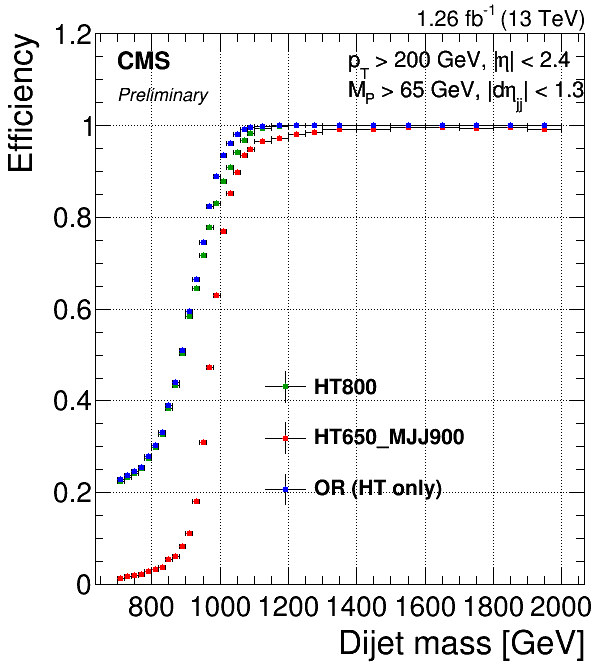
\includegraphics[width=0.4\textwidth]{figures/analysis/search1/AN-15-211//triggereffMjj-HT.png}
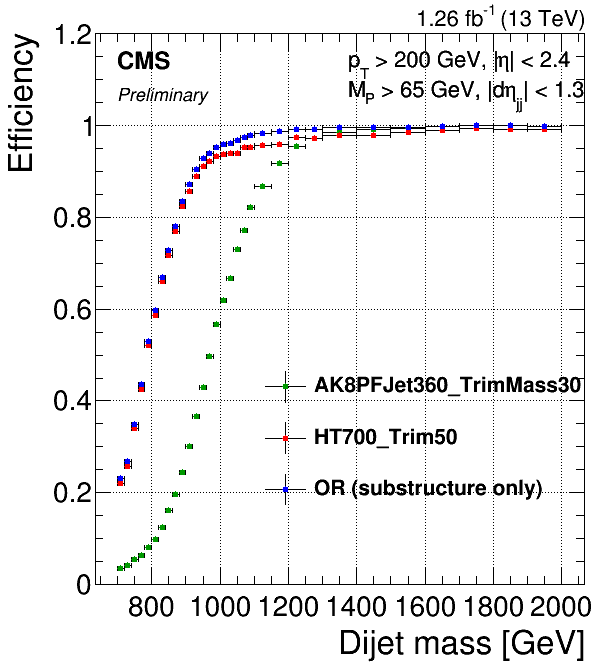
\includegraphics[width=0.4\textwidth]{figures/analysis/search1/AN-15-211//triggereffMjj-SUBST.png}\\
\caption{Efficiency for the inclusive triggers (left) and the grooming triggers (right) as a function of dijet invariant mass for jet pairs where one jet has a pruned mass larger than 65 GeV.}
\label{fig:searchI:HT-mjj-trigger}
\end{figure}

The real power of the grooming triggers become clear when adding them in OR with the \HT-based triggers. Figure~\ref{fig:searchI:trigger-fits} compares the trigger turn-on curves as a function of dijet invariant mass for jets passing one of the three inclusive triggers only, one of the grooming triggers only and when combining all of them. Here, one can see that the 99\% efficiency threshold is lowered by 75 \GeV when including the substructure triggers, once substructure is required at analysis level.
This allowed for the analysis to start at a dijet invariant mass of 1 TeV.

\begin{figure}[htb]
\centering
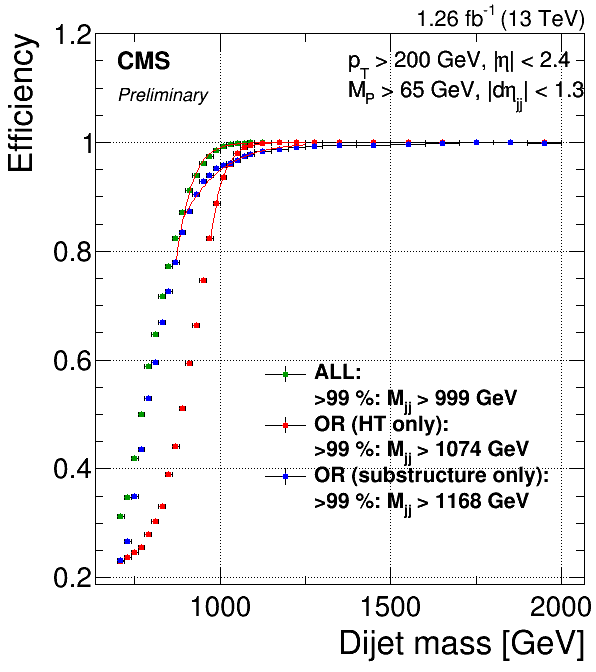
\includegraphics[width=0.4\textwidth]{figures/analysis/search1/AN-15-211/triggereffMjj-ALL.png}\\
\caption{Comparison of trigger efficiencies for jets passing one of the HT-triggers only (red), for jets passing one of the grooming-triggers only (blue) and for jets passing one of the HT-triggers or one of the grooming triggers (green). Here as a function of dijet invariant mass for all jet pairs passing loose selections and where one jet has a pruned mass larger than 65 GeV. The 99\% efficiency threshold is lowered by 75 \GeV when including substructure taggers. }
\label{fig:searchI:trigger-fits}
\end{figure}

As a measure of the performance of the grooming triggers, we have in addition looked at the trigger efficiencies as a function of the offline groomed mass (pruned and softdrop, see Sections~\ref{sec:objreco:pruning} and ~\ref{sec:objreco:softdrop}), for the grooming trigger with the lowest mass threshold (30 \GeV). This is shown in Figure~\ref{fig:searchI:grooming-mj-trigger}, where an additional cut on the jet transverse momentum of one of the jets of 600 GeV is required and no other mass cut is applied. The trigger plateau is reached for offline groomed-jet masses around 50 GeV, an impressively sharp turn-on for a trigger paths first test i data (as reference trigger for this study, the prescaled trigger \texttt{HLT\_PFJet320} was used). 

\begin{figure}[htb]
\centering
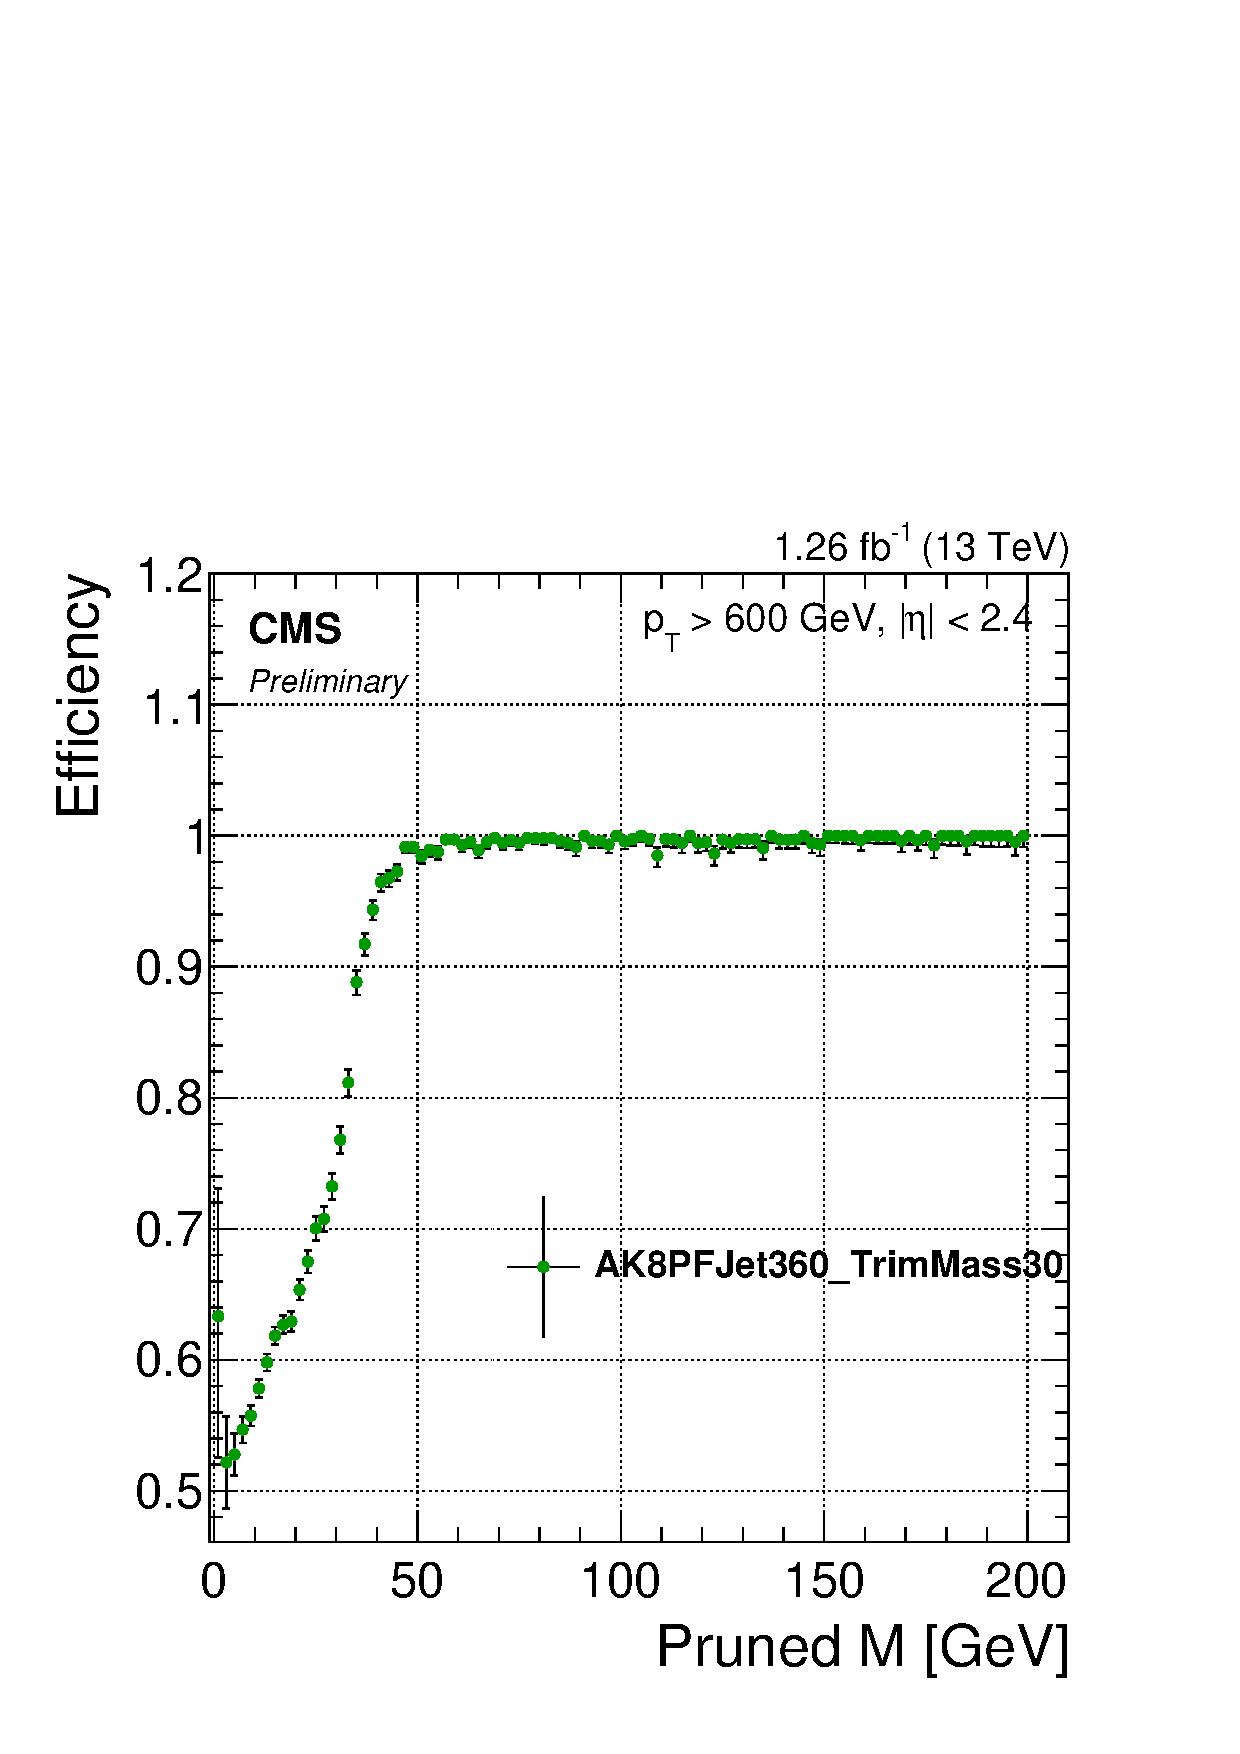
\includegraphics[width=0.4\textwidth]{figures/analysis/search1/AN-15-211//triggereff-prunedmass600.pdf}
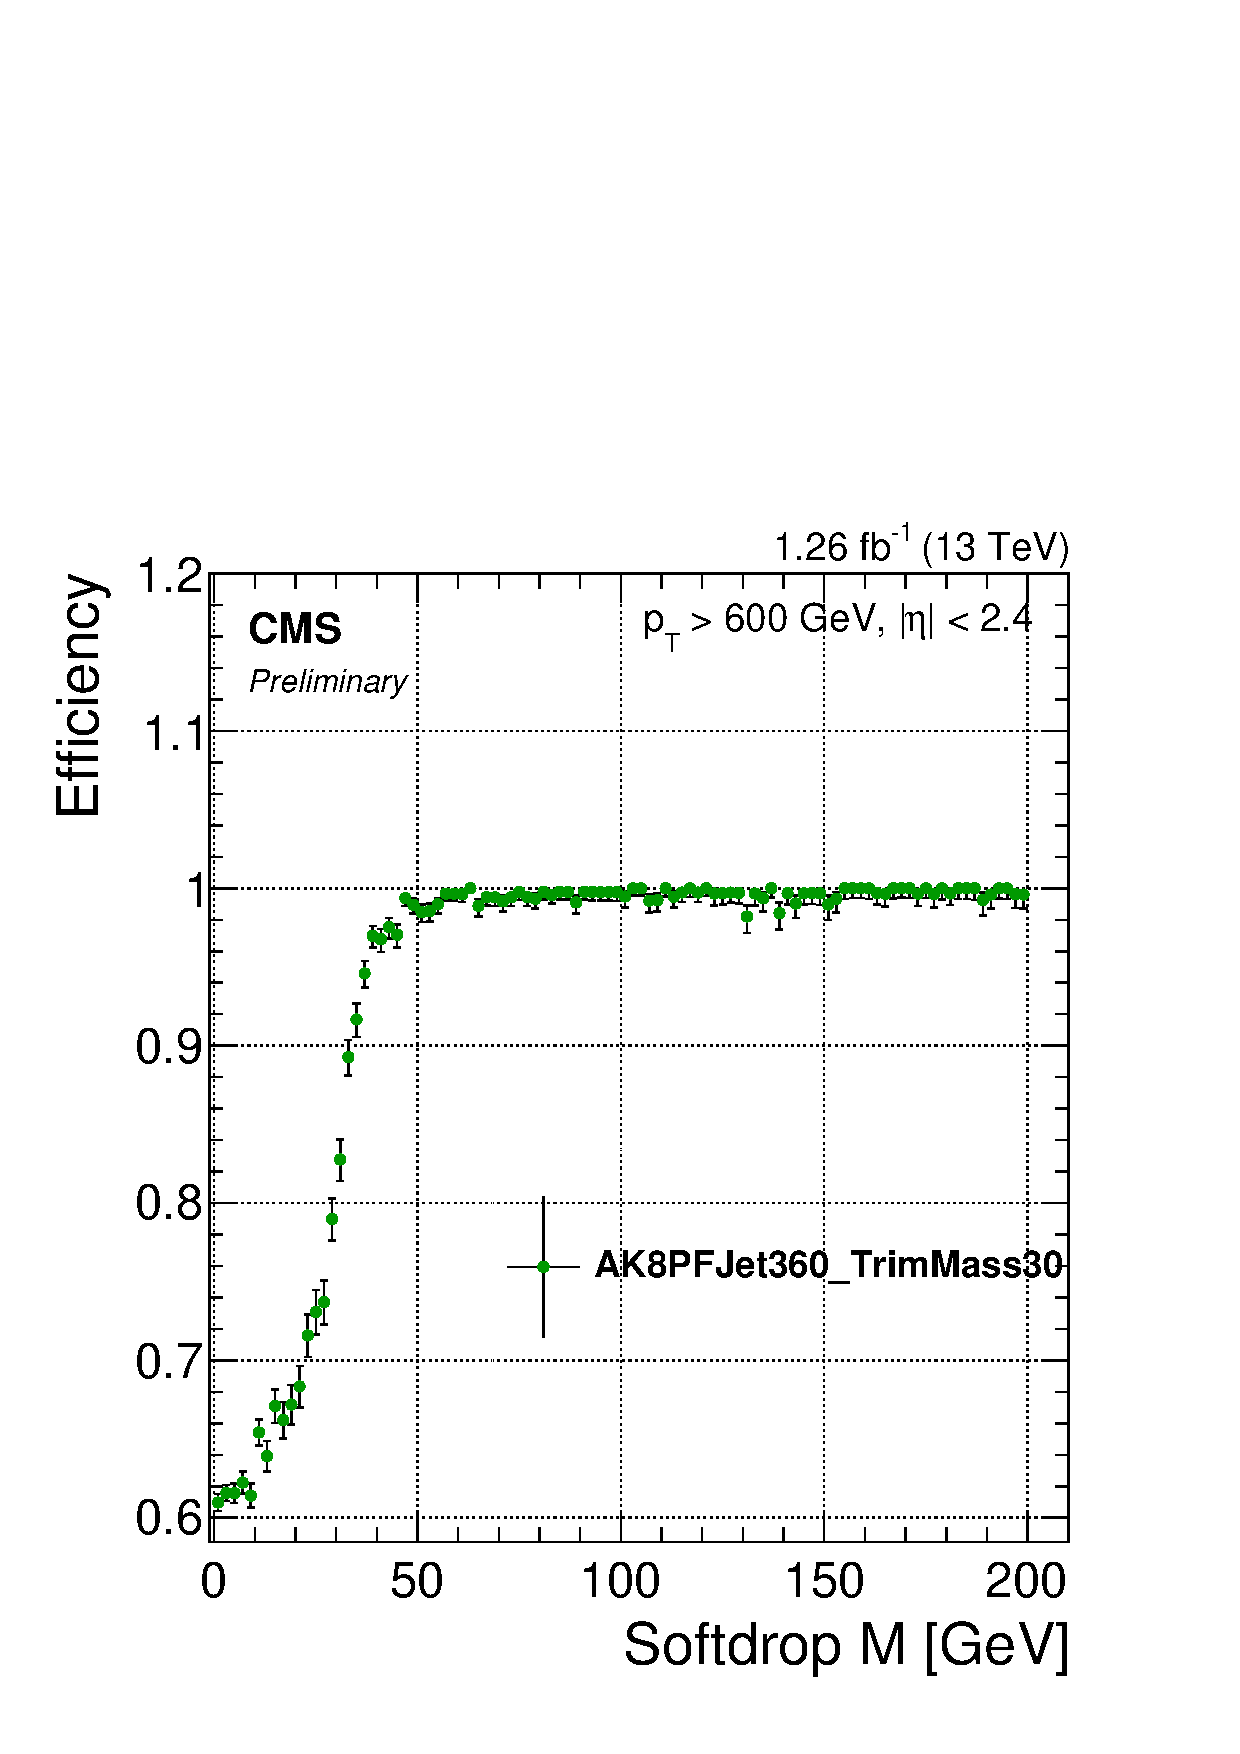
\includegraphics[width=0.4\textwidth]{figures/analysis/search1/AN-15-211//triggereff-sdmass.pdf}
\caption{Efficiency for the lowest threshold grooming trigger as a function of pruned-jet (left) and softdrop-jet (right) mass for jets with $\PT > \unit{600}{\GeV}$.}
\label{fig:searchI:grooming-mj-trigger}
\end{figure}




\subsubsection{Preselection} 
After trigger selections and the corresponding requirement of a dijet invariant mass above 1 \TeV to ensure a smoothy falling background, the process of maximizing the signal significance while keeping the background low can begin. This is done through a set of jet requirements. The jets used in this analysis are clustered with the anti-\kt{} jet clustering algorithm with a clustering parameter of $R=0.8$ (see Section ~\ref{sec:objreco:jets}) to allow containment of the full vector boson decay products. These jets are further required to pass certain jet identification requirements provided by the JetMET POG~\cite{jetID_JME}, in order to distinguish them from fake jets. These are as follows:
\begin{itemize}
\item Number of Constituents $> 1$, for all jet $\eta$
\item Neutral Hadron Energy Fraction $< 0.90$, for all jet $\eta$
\item Neutral EM Energy Fraction $< 0.90$, for all jet $\eta$
\item Charged Hadron Multiplicity $> 0$, for jet $|\eta| < 3.0$
\item Charged EM Energy Fraction $< 0.99$, for jet $|\eta| < 3.0$
\end{itemize} 
Jets are further corrected for nonlinearities in $\PT$ and rapidity using standard jet energy corrections at CMS as described in Ref.~\cite{jme_jinst} for $R$=0.8 anti-\kt{} jets.
As we know that a minimum transverse of 200 \GeV is required for the decay products of a \PW/\PZ to be fully contained within an R=0.8 jet, events are further selected by requiring at least two jets with $\PT > \unit{200}{\GeV}$. These are in addition required to be central, with an $|\eta| < 2.4$. \par
The two highest \PT jets in the event passing these criteria are selected as potential vector boson candidates.
As our main background is QCD multijet events, we further take advantage of the fact that the angular distribution between these, mainly t-channel, processes are very different from the s-channel signal processes under study. The QCD t-channel jets are mostly forwardly produced, with an opening angle with respect to the beam axis close to zero, while the signal jets are concentrated in the barrel region. We therefore require the jets to have a separation of $|\Delta\eta|<1.3$ in order to reduce the QCD multijets background.
The distribution of $|\Delta\eta|$ between the two highest-\PT jets for QCD as well as for different signal scenarios, is shown in Figure~\ref{fig:searchI:detaopt}

\begin{figure}[htb]
\centering
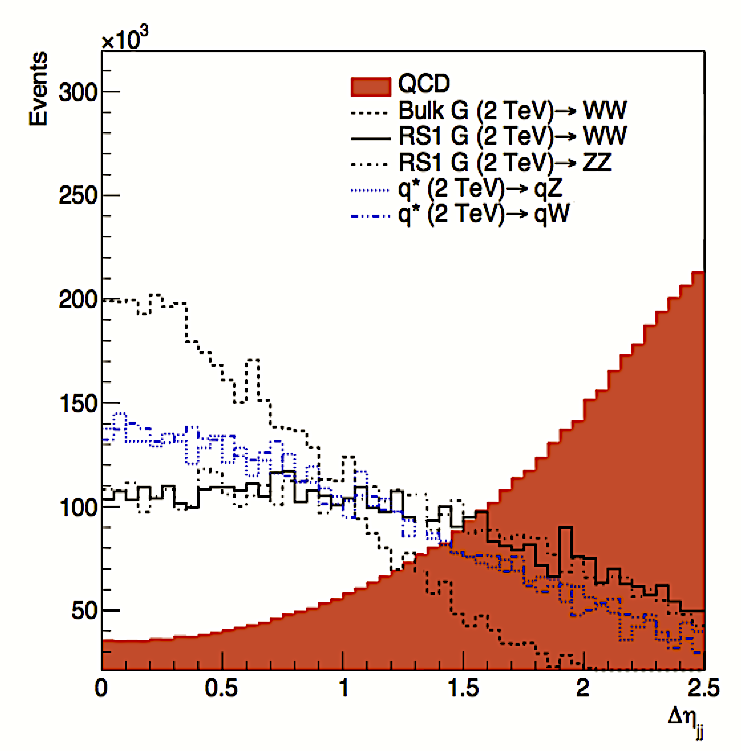
\includegraphics[width=0.4\textwidth]{figures/analysis/search1/misc/deta_opt.png}
\caption{ $|\Delta\eta|$  between the two highest-\PT jets for QCD jets and jets stemming from different signal scenarios.}
\label{fig:searchI:detaopt}
\end{figure}
 

A summary of the applied preselections is as follows:

\subsubsection{Vector boson tagging}

\subsection{Background modeling}
\label{sec:searchI:bkg}


